\chapter{Rational, real and complex numbers}\label{chapter:rationals}
{\small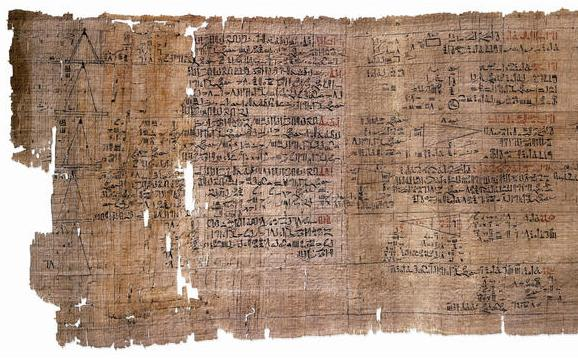
\includegraphics{Rhind_Mathematical_Papyrus.jpg}
A fragment of the Rhind papyrus, 1650BCE, containing ancient Egyptian calculations using rational numbers}\SubIndex{papyrus!Rhind}\SubIndex{Rhind papyrus}
\epigraph[author={Les Dawson}]{There is a remote tribe that worships the number zero. Is nothing sacred?}\SubIndex{Dawson, Les}\SubIndex{zero}
\section{Rational numbers}
A \emph{rational number}\define{rational!number}\define{number!rational} is a ratio of two integers, like
\[
\frac{2}{3}, \quad \frac{-7}{9}, \quad \frac{22}{-11}, \quad \frac{0}{2}.
\]
We also write them \(2/3, -7/9, 22/{-11}, 0/2\).
In writing \(\frac{2}{3}\), the number \(2\) is the \emph{numerator}\define{numerator}, and \(3\) is the \emph{denominator}\define{denominator}.
We can think of rational numbers two different ways: 
\begin{enumerate}
\item
Geometry: Divide up an interval of length \(b\) into \(c\) equal pieces.
Each piece has length \(b/c\).
\item
Algebra: a rational number \(b/c\) is just a formal expression we write down, with two integers \(b\) and \(c\), in which \(c\ne 0\).
We agree that any rational number \(\frac{b}{c}\) is equal to \(\frac{ab}{ac}\) for any integer \(a \ne 0\).
\end{enumerate} 
Of course, the two ideas give the same objects but the algebra approach is more elementary.
For example, we see that \(22/11=14/7\), because I can factor out:
\[
\frac{22}{11} = \frac{11 \cdot 2}{11 \cdot 1},
\]
and factor out
\[
\frac{14}{7} = \frac{7 \cdot 2}{7 \cdot 1}.
\]
Write any rational number \(\frac{b}{1}\) as simply \(b\), and in this way see the integers sitting among the rational numbers.

More generally, any rational number \(b/c\) can be simplified by dividing \(b\) and \(c\) by their greatest common divisor, and then changing the sign of \(b\) and of \(c\) if needed, to ensure that \(c > 0\); the resulting rational number is \emph{in lowest terms}.
\begin{problem}{rationals:lowest.terms}
Bring these rational numbers to lowest terms: \(224/82\), \(324/-72\), \(-\num{1000}/\num{8800}\).
\end{problem}
\begin{answer}{rationals:lowest.terms}
\(224/82=112/41\), \(324/-72=-9/2\), \(-\num{1000}/\num{8800}=-5/44\).
\end{answer}
Multiply rational numbers by
\[
\frac{b}{c} \frac{B}{C} = \frac{bB}{cC}.
\]
Similarly, divide a rational number by a \emph{nonzero} rational number as
\[
\frac{\frac{b}{c}}{\frac{B}{C}} = \frac{b}{c} \frac{C}{B}.
\]
Add rationals with the \emph{same denominator} as:
\[
\frac{b}{d} + \frac{c}{d} = \frac{b+c}{d}.
\]
The same for subtraction:
\[
\frac{b}{d} - \frac{c}{d} = \frac{b-c}{d}.
\]
But if the denominators don't match up, we rescale to make them match up:
\[
\frac{b}{c} + \frac{B}{C} = \frac{bC}{cC} + \frac{cB}{cC}.
\]
\begin{problem}{rationals:define.ops}
If we replace \(\frac{b}{c}\) by \(\frac{ab}{ac}\) and we replace \(\frac{B}{C}\) by \(\frac{AB}{AC}\), for some nonzero integers \(a,A\), prove that the result of computing out \(\frac{b}{c}+\frac{B}{C}\), \(\frac{b}{c}-\frac{B}{C}\) or \(\frac{b}{c}\frac{B}{C}\) only changes by scaling both numerator and denominator by the same nonzero integer.
Hence the arithmetic operations don't contradict our agreement that we declare \(\frac{b}{c}\) to equal \(\frac{ab}{ac}\).
\end{problem}
\begin{answer}{rationals:define.ops}
We can start by defining, for any pair of integers \((b,c)\) with \(c \ne 0\), and any pair of integers \((B,C)\) with \(C \ne 0\), a rational number  
\[
\frac{\beta}{\gamma}=(Cb+cB,cC).
\]
This is well defined, since \(cC \ne 0\).
If we replace \((b,c)\) by \((ab,ac)\) and replace \((B,C)\) by \((AB,AC)\), then we get rational number
\[
\frac{ACab+acAB}{acAC}=\frac{(Aa)(Cb+cB)}{(Aa)(Cc)}=\frac{Cb+cB}{Cc}
\]
unchanged.
So the resulting \(\beta/\gamma\) is independent of the choices of pairs, depending only on the rational numbers \(b/c\) and \(B/C\).
The other proofs are very similar.
\end{answer}
\begin{problem}{rationals:arithmetic}
By hand, showing your work, simplify
\[
\frac{2}{3}-\frac{1}{2}, \frac{324}{49} \cdot \frac{392}{81},
\frac{4}{5}+\frac{7}{4}.
\]
\end{problem}
\begin{answer}{rationals:arithmetic}
By hand, showing your work, simplify
\[
\frac{2}{3}-\frac{1}{2}=\frac{1}{6}, \frac{324}{49} \cdot \frac{392}{81}=32,
\frac{4}{5}+\frac{7}{4}=\frac{51}{20}.
\]
\end{answer}
\begin{lemma}
The number \(\sqrt{2}\) is irrational.
(To be more precise, no rational number squares to \(2\).)
\end{lemma}
\begin{proof}
If it is rational, say \(\sqrt{2}=\frac{b}{c}\), then \(c \sqrt{2}=b\), so squaring gives \(c^2 \cdot 2 = b^2\).
Every prime factor in \(b\) occurs twice in \(b^2\), so the prime factorization of the right hand side has an even number of factors of each prime.
But the left hand side has an odd number of factors of \(2\), since \(c^2\) has an even number, but there is another factor of \(2\) on the left hand side.
This contradicts uniqueness of prime factorization.
\end{proof}
\begin{problem}{rationals:square.roots}
Suppose that \(N\) is a positive integer.
Prove that either \(\sqrt{N}\) is irrational or \(N\) is a \emph{perfect square}\define{perfect square}, i.e. \(N=n^2\) for some integer \(n\).
\end{problem}
\begin{problem}{rationals:square.roots.2}
Prove that there are no rational numbers \(x\) and \(y\) satisfying \(\sqrt{3}=x+y\sqrt{2}\).
\end{problem}
\begin{answer}{rationals:square.roots.2}
If \(\sqrt{3}=x+y\sqrt{2}\), square both sides to get
\[
3 = x^2+2xy\sqrt{2}+2y^2.
\]
If \(y\ne 0\), we can solve for \(\sqrt{2}\) as a rational expression in \(x,y\), so a rational number, a contradiction.
Hence \(y=0\) and \(\sqrt{3}=x\) is rational, a contradiction.
\end{answer}
A rational number is \emph{positive}\define{positive!rational number} if it is a ratio of positive integers.
We write \(x > y\) to mean that \(x-y\) is positive, and similarly define \(x<y\), \(x\le y\), and so on.
\begin{problem}{rationals:factorization}
Prove that every positive rational number has a unique expression in the form
\[
\frac{p_1^{\alpha_1} p_2^{\alpha_2} \dots p_k^{\alpha_k}}%
{q_1^{\beta_1} q_2^{\beta_2} \dots q_{\ell}^{\beta_{\ell}}}
\]
where
\[
p_1, p_2, \dots, p_k, q_1, q_2, \dots, q_{\ell}
\] 
are prime numbers, all different, with \(p_1 < p_2 < \dots < p_k\) and \(q_1 < q_2 < \dots < q_{\ell}\) and
\[
\alpha_1, \alpha_2, \dots, \alpha_k,
\beta_1, \beta_2, \dots, \beta_{\ell}
\]
are positive integers.
For example
\[
\frac{234}{16}=\frac{3^2 \cdot 13}{2^3}.
\]
\end{problem}
\begin{answer}{rationals:factorization}
By definition, every positive rational number is a ratio \(b/c\) with \(b\) and \(c\) positive.
We can divide out their greatest common divisor to arrange that \(b,c\) are coprime.
Take the prime factorization of \(b\), and that of \(c\).
As they are coprime, no prime occurs in both factorizations. 
\end{answer}
\begin{problem}{rationals:properties}
Of the various laws of addition and multiplication and signs for integers, which hold true also for rational numbers?
\end{problem}
The most important property that rational numbers have, that integers don't, is that we can divide any rational number by any nonzero rational number.

\section{Real numbers}
\epigraph[author={J.A.~Froude}]{Order is an exotic in Ireland. It has been imported from England but will not grow. It suits neither soil nor climate.}
Think of the rational numbers geometrically, so that \(b/c\) is the length of each piece when a rod of length \(b\) is cut into \(c\) equal lengths.
Draw an straight line, infinite in both directions, and mark a point \(0\) on it.
Then mark at point \(1\) at 1 unit of distance from \(0\), and so on marking all of the integers to form a \emph{number line}.\define{number line}
The points of this continuous number line are the \emph{real numbers}.
This physical definition doesn't make it possible to prove anything about the real numbers.

The rational numbers are insufficient for algebra: they have no \(\sqrt{2}\).
Imagine taking all positive rational numbers \(b/c\) for which \(b^2/c^2 > 2\).
Thinking geometrically, drawing a number line:
\begin{center}
\documentclass[tikz]{standalone}
\usepackage{xparse}
\colorlet{curveZero}{gray!85}
\colorlet{curveOne}{blue!60}
\definecolor{curveOneColor}{rgb}{.6,0,0}
\colorlet{curveTwo}{brown!50!gray}
\colorlet{curveThree}{green!40!gray}
\colorlet{curveFour}{red!50!gray}
\NewDocumentCommand\DrawDotInPlot{O{}mmO{}}%
{%
\fill[gray!15,draw=gray] (axis cs:{#2},{#3}) circle [radius=1.6pt] node[above,black,#4] {\(#1\)};%
}%
\NewDocumentCommand\DrawDot{O{}mmO{}}%
{%
\fill[gray!20,draw=gray] ({#2},{#3}) circle (1.6pt) node[above,black,#4] {\(#1\)};%
}%
\NewDocumentCommand\DrawNode{O{}m}%
{%
\fill[gray!20,draw=gray] (#2) circle (1.6pt) node[above,black] {\(#1\)};%
}%
\NewDocumentCommand\DrawDotThreeD{O{}mmmO{}}%
{%
\fill[gray!20,draw=gray] ({#2},{#3},{#4}) circle (1.6pt) node[above,black,#5] {\(#1\)};%
}%
\colorlet{axisColor}{gray!50}
\tikzstyle{shapeZero}=[fill=curveZero,opacity=.4]
\tikzstyle{shapeOne}=[fill=curveOne,opacity=.4]
\tikzstyle{shapeTwo}=[fill=curveTwo,opacity=.4]
\tikzstyle{shapeThree}=[fill=curveThree,opacity=.4]
\tikzstyle{groupElementLabel}=[minimum size=2.4em]
\tikzstyle{groupElement}=[minimum size=2.4em,shapeZero,draw=curveZero]
\tikzstyle{cosetOne}=[minimum size=2.4em,shapeOne,draw=curveOne]
\tikzstyle{cosetTwo}=[minimum size=2.4em,shapeTwo,draw=curveTwo]


\begin{document}
\begin{tikzpicture}
\draw[axisColor](-1,0) -- (3,0);
\draw[very thick,axisColor]({sqrt(2)},0) -- (3,0);
\DrawDot[\sqrt{2}]{sqrt(2)}{0}
\end{tikzpicture}
\end{document}

\end{center}
Our rational numbers sit along the line getting very close to the circled point of the line, which should be the point \(\sqrt{2}\).
But there is no rational number there.
From now on, we assume that the reader is familiar with the real numbers and their basic properties; see \cite{Spivak:2006} for the complete story of real numbers.
\begin{problem}{real:fast.accurate.2}
Given numbers \(a,b,c,x\), note that \(ax^2+bx+c=(ax+b)x+c\).
But if we plug in and compute, which expression is faster to compute with?
Suppose that we compute approximately, and every addition and multiplication produces some error; which expression is more accurate?
\end{problem}
\begin{problem}{real:rounding}
If you add first and then round to some number of decimals, and I round first and then add, how far apart can our results be? How close? What if we subtract instead of adding?
Or if we multiply?
\end{problem}
\begin{problem}{real:point.nine}
Explain why \(1=.99999\dots\).
How many different decimal expansions can a real number have, and which real numbers have that many?
\end{problem}

\section{Complex numbers}
\epigraph[author={Paul Painlev\'e}, source={Analyse des travaux scientifiques}, translation={The shortest and easiest path between any two facts about the real domain often passes through the complex domain.}]{Entre deux vérités du domaine réel, le chemin le plus facile et le plus court passe bien souvent par le domaine complexe.}%
\SubIndex{Painlev\'e, Paul}
Just as the rational numbers have a deficiency, no \(\sqrt{2}\), so the real numbers have a deficiency: no \(\sqrt{-1}\).
We can fix this by introducing the complex numbers.
Here are two definitions:
\begin{enumerate}
\item
\emph{Algebra:} We agree to play a game, where we write down algebraic expressions in real numbers and in an abstract variable \(i\), but we treat the symbol \(i\) according to the following rule.
Whenever we see two copies of \(i\) multiplied together (or we see \(i^2\)) appear anywhere, we are allowed to wipe them out and replace with \(-1\), and vice versa when we see a \(-1\) we can replace it with an \(i^2\).
We force by hand the existence of a \(\sqrt{-1}\) by forcing the abstract symbol \(i\) to be \(\sqrt{-1}\).
\item
\emph{Geometry:} We draw the usual \(x,y\) axes on the plane.
We pretend that each point of the plane represents a single number, which we write as \(z=x+yi\) to represent the point \((x,y)\).
If we have two points, \(z=x+yi\) and \(Z=X+Yi\), we add them by the rule:
\[
z+Z=(x+X)+(y+Y)i
\]
and multiply them by the rule:
\[
zZ=(xX-yY)+(xY+yX)i.
\]
For example, 
\[
(2+4i)(3-i)=(2\cdot 3 + 4\cdot 1)+(-2+4\cdot 3)i=10+10i.
\]
\end{enumerate}
It isn't at all clear that these two games we can play arrive at the same result.
Note that the rule for multiplication seems to come out of the air in the geometric theory, but in the algebraic theory it is just what you get by expanding out both sides and insisting that \(i^2=-1\).
Algebra is in this respect clearly superior. 
But the geometric approach makes very precise what sort of objects we are really dealing with, so we will use it as our definition.

Just like with rational numbers, if a complex number \(z=x+yi\) is not zero, or in other words \(x\) and \(y\) are not both zero, then it has a reciprocal
\[
\frac{1}{z} = \frac{x-yi}{x^2+y^2}.
\]
\begin{problem}{rationals:recip.c}
Check that this is a reciprocal.
Why is it defined?
\end{problem}
\emph{Complex conjugation}\define{complex conjugation} is the operation taking \(z=x+yi\) to \(\bar{z}\defeq x-iy\).
\begin{problem}{rationals:conjugate.real}
Prove that a complex number \(z\) is a real number just when \(z=\bar{z}\). 
\end{problem}
\begin{problem}{rationals:conjugate}
Prove that addition, subtraction, multiplication and division of complex numbers passes through conjugation:
\begin{align*}
\overline{z+w}&=\bar{z}+\bar{w}, \\
\overline{z-w}&=\bar{z}-\bar{w}, \\
\overline{zw}&=\bar{z} \, \bar{w}, \\
\overline{\pr{\frac{z}{w}}}&=\frac{\bar{z}}{\bar{w}},
\end{align*}
for any complex numbers \(z\) and \(w\).
Explain by induction why, for any polynomial \(p(z)\) with real number coefficients,
\[
\overline{p(z)}=p\of{\bar{z}},
\]
for any complex number \(z\).
\end{problem}
The \emph{norm}\define{norm} or \emph{modulus}\define{modulus} of a complex number \(z=x+yi\) is the real number \(|z|\defeq\sqrt{x^2+y^2}\)\Notation{(z)}{\lengthForNotationIndex{z}}{modulus of a complex number}.
\begin{problem}{rationals:norm}
Prove that \(z\bar{z}=|z|\) for any complex number \(z\).
\end{problem}

\section{Sage}
\epigraph[author={Friedrich Nietzsche}, source={\"Uber Wahrheit und L\"uge im aussermoralischen Sinne}, translation={What, then, is truth? A mobile army of metaphors, metonyms, and anthropomorphisms---in short, a sum of human relations, which have been enhanced, transposed, and embellished poetically and rhetorically, and which after long use seem firm, canonical, and obligatory to a people: truths are illusions about which one has forgotten that this is what they are; metaphors which are worn out and without sensuous power; coins which have lost their pictures and now matter only as metal, no longer as coins.}]{Was ist also Wahrheit? Ein bewegliches Heer von Metaphern, Metonymien, Anthropomorphismen, kurz eine Summe von menschlichen Relationen, die, poetisch und rhetorisch gesteigert, \"ubertragen, geschm\"uckt wurden, und die nach langem Gebrauch einem Volke fest, kanonisch und verbindlich d\"unken: die Wahrheiten sind Illusionen, von denen man vergessen hat, da\ss sie welche sind, Metaphern, die abgenutzt und sinnlich kraftlos geworden sind, M\"unzen, die ihr Bild verloren haben und nun als Metall, nicht mehr als M\"unzen, in Betracht kommen.}%
\SubIndex{Nietzsche, Friedrich}\SubIndex{Uber Wahrheit und Luge im aussermoralischen Sinne@\"Uber Wahrheit und L\"uge im aussermoralischen Sinne}%
Sage represents numbers in two different ways: as exact symbolic expressions, or as a finite decimal approximation (often called a \emph{numeric} or \emph{floating point} representation). 
For example we compute \(\frac{7}{2}+\frac{5}{3}\) symbolically as
\begin{sageblock}
7/2+5/3
\end{sageblock}
yielding \(\sage{7/2+5/3}\).
We can also play with irrational numbers symbolically: represent \(\sqrt{27}\) as
\begin{sageblock}
sqrt(27)
\end{sageblock}
which sage simplifies to yield \(\sage{sqrt(27)}\).

We will \emph{never} use decimal approximations in this class (please don't), but here is how you can use them if you wish.
By writing out a number with a decimal point, we are asking sage to approximate numerically, keeping only some number of decimals accuracy:
\begin{sageblock}
sqrt(27.0)
\end{sageblock}
yields \(\sage{sqrt(27.0)}\).
If we want to ask sage to give us a particular number of decimal places accuracy in a decimal approximation of a symbolic expression, say \(50\) decimals:
\begin{sageblock}
numerical_approx(pi, digits=50)
\end{sageblock}
yields 
\[
\sage{numerical_approx(pi, digits=50)}.
\]

To use complex numbers, try 
\begin{sageblock}
z=3+4*i
real_part(z)
\end{sageblock}
yielding \(3\), the real part, while \verb!imag_part(z)! yields \(4\).


